\documentclass{beamer}
\usepackage{array}
\usepackage{graphicx}
\usepackage{subfigure}
\usepackage{hyperref}
\hypersetup{colorlinks=true}
\mode<presentation>
{
	\usetheme{Madrid}       % or try default, Darmstadt, Warsaw, ...
	\usecolortheme{default} % or try albatross, beaver, crane, ...
	\usefonttheme{serif}    % or try default, structurebold, ...
	\setbeamertemplate{navigation symbols}{}
	\setbeamertemplate{caption}[numbered]
} 

\usepackage[english]{babel}
\usepackage[utf8x]{inputenc}

% Here's where the presentation starts, with the info for the title slide
\title[\textcolor{white}{Supervisor: Megan Oliver}]{Modelling Host-Parasite Relationships with Multiple Infection}
\author{Jiaze Sun}
\date{September 21, 2022}

\begin{document}
	
	\begin{frame}
		\titlepage
	\end{frame}
	
	\section{Introduction}
	\subsection{Introduction}
	\begin{frame}{Introduction}
		\begin{itemize}
			\item In 2021, Scientists in Brazil reported evidence of SARS-CoV-2 multiple infection by distinct strains.
		\begin{figure}[ht]
			\label{Figure 1}
			\begin{center}
				\includegraphics[width=330pt]{"Co-infection_of_Different_Covid_Lineages.jpg"}
			\end{center}
			\caption{\tiny Population structure and intra-host variation amended from Francisco Jr et al., \href{https://doi.org/10.1016/j.virusres.2021.198345}{Pervasive transmission of E484K and emergence of VUI-NP13L with evidence of SARS-CoV-2 co-infection events by two different lineages in Rio Grande do Sul, Brazil}, 2021, p.198345-198345. Used under a UK Copyright Exception.}
		\end{figure}
		\end{itemize}
	\end{frame}

	\begin{frame}{Introduction}
		\begin{itemize}
			\item \textbf{Strain} here refers to a parasite population with a particular characteristic (known as trait).
			\vspace{1em}
			\item Naturally, humans and animals (known as hosts) tend to be infected by different strains of the same parasite species, resulting from separate infecting events or a high mutation rate. 
		\end{itemize}
	\end{frame}
	
	\subsection{Multiple Infection}
	\begin{frame}{Multiple Infection}
		\begin{itemize}
			\item Multiple infection: (in my work it is defined to be) infection caused by multiple strains of the same parasite species. 
			\vspace{1em}
			\item Three basic theoretical frameworks have been used to study multiple infection:
			\vspace{1em}
			\begin{itemize}
				\item \textbf{Superinfection}: a parasite strain infects hosts alone but can be displaced by one another based on strain traits,
				\item \textbf{Co-infection}: two or more parasite strains can infect each host simultaneously,
				\item \textbf{Kin Selection}: the relatedness of strains and the fact that the collective action of co-infecting strains may affect overall virulence are considered.
			\end{itemize}
		\end{itemize}
	\end{frame}

	\subsection{Virulence}
	\begin{frame}{Virulence}
		\begin{itemize}
			\item Virulence: the damage to host fitness caused by infection.
			\vspace{1em}
			\item In the model, virulence is measured as host mortality rate caused by the infection.
		\end{itemize}
	\end{frame}
	
	\section{The Model}
	\begin{frame}{Notations}
		\begin{table}
		\begin{tabular}{c l}
			\hline
			$\mu$\ \  & Baseline mortality rate \\
			\hline
			$S$\ \  & Density of susceptible hosts \\
			\hline
			$I_1$\ \ & Density of hosts being singly infected\\
			\hline
			$D_{11}$\ \ & Density of hosts being co-infected\\
			\hline
			$\rho$\ \ & Host input (birth rate)\\
			\hline
			$\alpha_1$\ \ & Virulence of a host being singly infected\\
			\hline
			$\alpha_{11}$\ \ & Virulence of a host being co-infected\\
			\hline
			$\beta_1$\ \ & Transmission rate in single infection\\
			\hline
			$\beta_{11}$\ \ & Transmission rate of the strain in a host being co- infected\\
			\hline
			$\sigma_S$\ \ & Vulnerability of susceptible hosts to infection\\
			\hline
			$\sigma_I$\ \ & Vulnerability of infected hosts to a new infection\\
			\hline
			$\lambda_1$\ \ & The force of infection of the strain\\
		\end{tabular}
		\end{table}
		\begin{itemize}
			\item the force of infection of the strain, $\lambda_1$, is defined as $\lambda_1\ =\ \beta_1I_1 + \beta_{11}D_{11}$.
		\end{itemize}
	\end{frame}

	\begin{frame}{The Model}
		\begin{itemize}
			\item The population dynamics of the strain in a co-infection situation can be governed by the following equations:
		\begin{align}
			\frac{dS}{dt}\ &=\ \rho -\mu S -\sigma_S\lambda_1S,\\
			\frac{dI_1}{dt}\ &=\ \sigma_S\lambda_1S -(\mu + \alpha_1+\sigma_I\lambda_1)I_1,\\
			\frac{dD_{11}}{dt}\ &=\ \sigma_I\lambda_1I_1 - (\mu+\alpha_{11})D_{11},
		\end{align}
		\begin{figure}[ht]
			\label{Figure 2}
			\begin{center}
				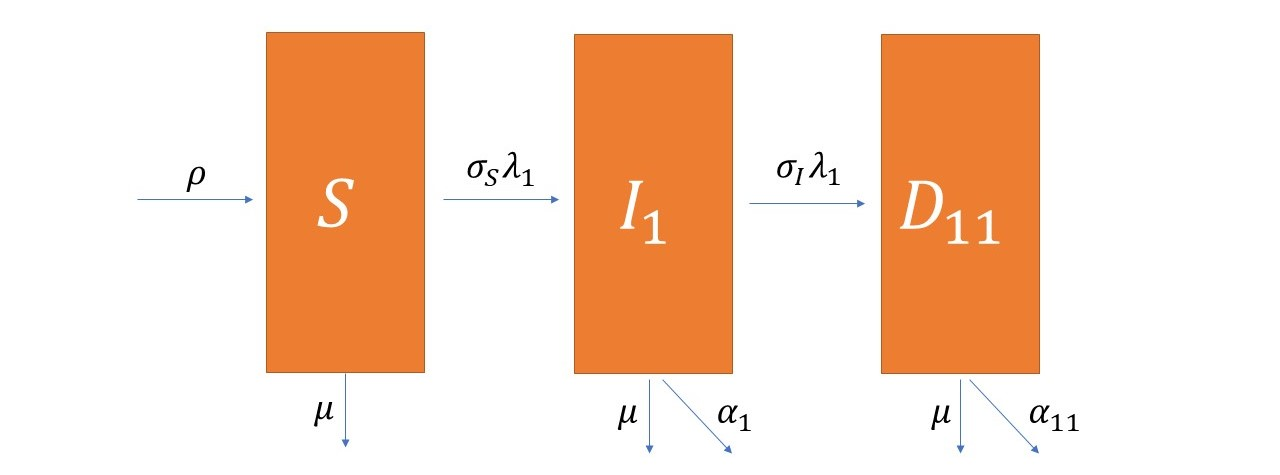
\includegraphics[width=230pt]{model.jpg}
			\end{center}
			\caption{Schematic diagram of the model.}
		\end{figure}
		\end{itemize}
	\end{frame}

	\section{The model with trade-off}
	\subsection{The Trade-off}
	\begin{frame}{The Trade-off}
		\begin{itemize}
			\item \textbf{The trade-off between transmission and virulence}: increasing parasite abundance can increase transmission but also may increase host death. 
			\vspace{1em}
			\item Mathematically, mortality rate caused by infection  can be made an increasing function of transmission rate. 
		\end{itemize}
	\end{frame}

	\subsection{The trade-off function}
	\begin{frame}{The trade-off function}
		\begin{itemize}
			\item The trade-off function takes the form
		\vspace{2em}
		\begin{equation}
			\alpha(\beta)\ =\ \alpha(\beta^{\ast})-\frac{\alpha^{\prime}(\beta^{\ast})^2}{\alpha^{\prime\prime}(\beta^{\ast})}\left[1-\exp\left(\frac{\alpha^{\prime\prime}(\beta^{\ast})(\beta-\beta^{\ast})}{\alpha^{\prime}(\beta^{\ast})}\right)\right].
		\end{equation}
		\end{itemize}
	\end{frame}

	\begin{frame}{The trade-off function}
		\begin{figure}[ht]
			\label{Figure 3}
			\begin{center}
				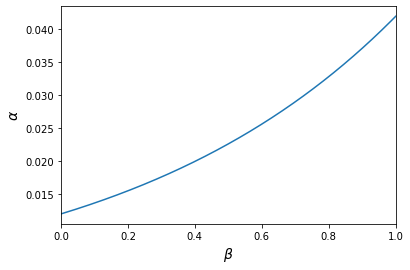
\includegraphics[width=250pt]{graph_of_trade_off_function.jpg}
			\end{center}
			\caption{Graph of the trade-off function, with parameters fixed as follows: $\beta^{\ast}\ =\ 0.4$, $\alpha(\beta^{\ast})\ =\ 0.02$, $\alpha^{\prime}(\beta^{\ast})\ =\ 0.025$, $\alpha^{\prime\prime}(\beta^{\ast})\ =\ 0.03$.}
		\end{figure}
	\end{frame}

	\subsection{Results}
	\begin{frame}{Results}
		\begin{itemize}
			\item When the population dynamics reach equilibrium, there are 3 scenarios of interest: \textbf{existence of both infected host types}, \textbf{disease-free} and \textbf{single infection only}.
		\end{itemize}
	\end{frame}
	
	\begin{frame}{Scenario I: Existence of both infected host types}
		\begin{figure}[ht]
			\label{Figure 4}
			\begin{center}
				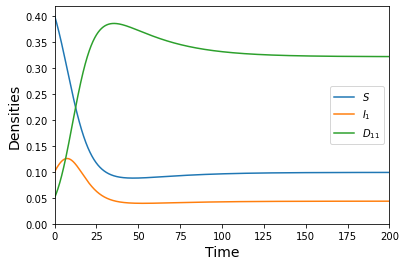
\includegraphics[width=220pt]{coexistence_of_singly_infected_and_coinfected_hosts.jpg}
			\end{center}
			\caption{Coexistence of singly infected and co-infected hosts, with parameters $\rho\ =\ \mu\ =\ 0.012$, $\beta_1\ =\ \beta_{11}\ =\ 0.3$, $\sigma_S\ =\ 1$, $\sigma_I\ =\ 2$.}
		\end{figure}
	\end{frame}

	\begin{frame}{Scenario II: Disease-free}
		\begin{itemize}
			\item The disease-free case may occur when the transmission rate is too low or,
			\vspace{1em}
			\begin{figure}[ht]
				\label{Figure 5}
				\begin{center}
					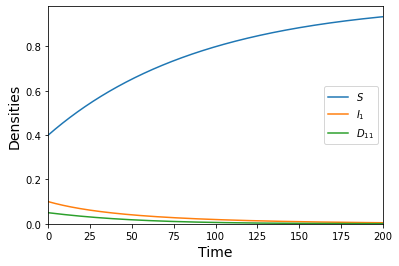
\includegraphics[width=220pt]{disease-free_with_low_transmission_rate.jpg}
				\end{center}
				\caption{Disease-free case with low transmission rate, with parameter $\rho\ =\ \mu\ =\ 0.012$, $\beta_1\ =\ \beta_{11}\ =\ 0.01$, $\sigma_S\ =\ 1$, $\sigma_I\ =\ 2$.}
			\end{figure}
		\end{itemize}
	\end{frame}

	\begin{frame}{Scenario II: Disease-free}
		\begin{itemize}
			\item when the background mortality rate is too high or,
			\vspace{1em}
			\begin{figure}[ht]
				\label{Figure 6}
				\begin{center}
					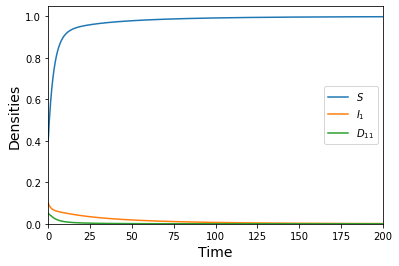
\includegraphics[width=220pt]{disease-free_with_very_high_background_mortality_rate.jpg}
				\end{center}
				\caption{Disease-free case with high background mortality rate, with parameter $\rho\ =\ \mu\ =\ 0.3$, $\beta_1\ =\ \beta_{11}\ =\ 0.3$, $\sigma_S\ =\ 1$, $\sigma_I\ =\ 2$.}
			\end{figure}
		\end{itemize}
	\end{frame}

	\begin{frame}{Scenario II: Disease-free}
		\begin{itemize}
			\item when the vulnerability of susceptible hosts is too low.
			\vspace{1em}
			\begin{figure}[ht]
				\label{Figure 7}
				\begin{center}
					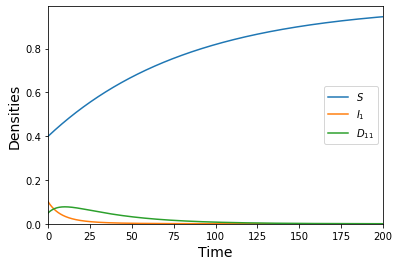
\includegraphics[width=220pt]{disease-free_with_low_sv.jpg}
				\end{center}
				\caption{Disease-free case with low vulnerability of susceptible host, with parameter $\rho\ =\ \mu\ =\ 0.012$, $\beta_1\ =\ \beta_{11}\ =\ 0.3$, $\sigma_S\ =\ 0.001$, $\sigma_I\ =\ 2$.}
			\end{figure}
		\end{itemize}
	\end{frame}

	\begin{frame}{Scenario III: Single infection only}
		\begin{itemize}
			\item The single-infection-only case may occur when it is hard for singly infected hosts to be infected again, i.e. the vulnerability of infected hosts is low.
			\vspace{1em}
		\begin{figure}[ht]
			\label{Figure 8}
			\begin{center}
				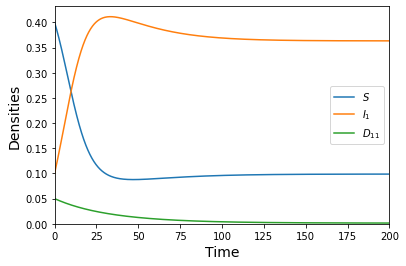
\includegraphics[width=220pt]{single_infection_only.jpg}
			\end{center}
			\caption{Single-infection-only case, with parameter $\rho\ =\ \mu\ =\ 0.012$, $\beta_1\ =\ \beta_{11}\ =\ 0.3$, $\sigma_S\ =\ 1$, $\sigma_I\ =\ 0.001$.}
		\end{figure}
		\end{itemize}
	\end{frame}
	
	\section{Extension}
	\subsection{Extension: Hosts vulnerability}
	\begin{frame}{Extension: Hosts vulnerability}
		\begin{itemize}
			\item $\sigma_S$ and $\sigma_I$: two new parameters which quantify the vulnerability of susceptible and infected hosts to a new infection.
		\end{itemize}
	\end{frame}

	\begin{frame}{Extension: Hosts vulnerability}
		\begin{itemize}
			\item The proportion of co-infected hosts decreases (increases) if the infected hosts are less (more) vulnerable to further infection.
			\vspace{1em}
			\begin{figure}[htbp]
				\label{Figure 9}
				\centering
				\subfigure[]{
					\begin{minipage}{0.3\columnwidth}
						\centering
						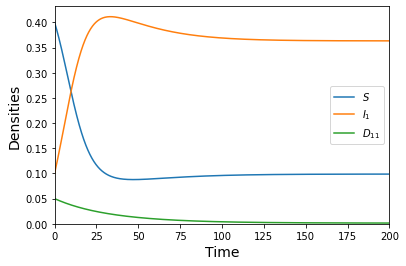
\includegraphics[width=100pt]{1_small.jpg}
					\end{minipage}
				}\subfigure[]{
					\begin{minipage}{0.3\columnwidth}
						\centering
						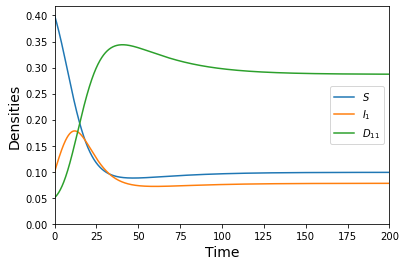
\includegraphics[width=100pt]{1_1.jpg}
					\end{minipage}
				}\subfigure[]{
					\begin{minipage}{0.3\columnwidth}
						\centering
						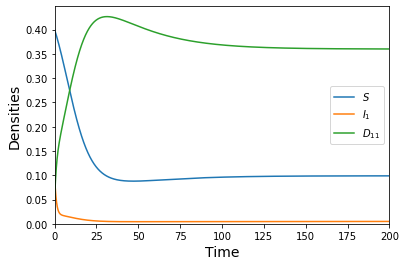
\includegraphics[width=100pt]{1_high.jpg}
					\end{minipage}
				}
				\caption{(a): $\sigma_S\ =\ 1$, $\sigma_I\ =\ 0.001$; (b): $\sigma_S\ =\ 1$, $\sigma_I\ =\ 1$; (c): $\sigma_S\ =\ 1$, $\sigma_I\ =\ 20$.}
			\end{figure}
		\end{itemize}
	\end{frame}

	\begin{frame}{Extension: Hosts vulnerability}
		\begin{itemize}
			\item The fraction of susceptible hosts increases (decreases) as the vulnerability of susceptible hosts decreases (increases).
			\vspace{1em}
			\begin{figure}[htbp]
				\label{Figure 10}
				\centering
				\subfigure[]{
					\begin{minipage}{0.3\columnwidth}
						\centering
						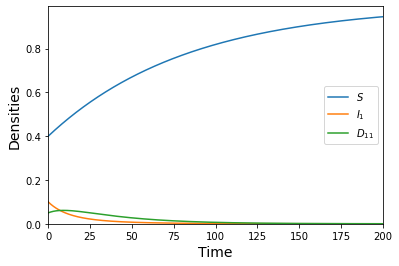
\includegraphics[width=100pt]{small_1.jpg}
					\end{minipage}
				}\subfigure[]{
					\begin{minipage}{0.3\columnwidth}
						\centering
						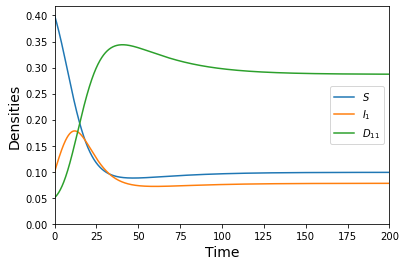
\includegraphics[width=100pt]{1_1.jpg}
					\end{minipage}
				}\subfigure[]{
					\begin{minipage}{0.3\columnwidth}
						\centering
						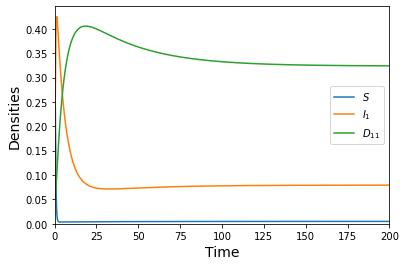
\includegraphics[width=100pt]{high_1.jpg}
					\end{minipage}
				}
				\caption{(a): $\sigma_S\ =\ 0.001$, $\sigma_I\ =\ 1$; (b): $\sigma_S\ =\ 1$, $\sigma_I\ =\ 1$; (c): $\sigma_S\ =\ 20$, $\sigma_I\ =\ 1$.}
			\end{figure}
		\end{itemize}
	\end{frame}

	\subsection{Extension: Micro-parasite vs. Macro-parasite}
	\begin{frame}{Extension: Micro-parasite vs. Macro-parasite}
		\begin{itemize}
			\item \textbf{Micro-parasites}: $D_{11}$ hosts resemble singly infected host, and $\alpha_{11}$ is the same as virulence caused by single infection,
			\item \textbf{Macro-parasites}: $D_{11}$, the density of hosts being co-infected, can be regarded as hosts with a double parasite load.
			\vspace{1em}
			\item In the analysis above, it is assumed that the parasite is micro-parasite. For the macro-parasite, the population dynamics does not vary greatly from that in micro-parasite case, i.e. it also has the similar three scenarios.
		\end{itemize}
	\end{frame}

	\subsection{Extension: Model with recovery}
	\begin{frame}{Extension: Model with recovery}
		\begin{itemize}
			\item Assume that both the singly infected and co-infected hosts can recover to susceptible class with recovery rate $\gamma_1$ and $\gamma_{11}$ respectively, and can be reinfected.
		\end{itemize}
	\end{frame}

	\begin{frame}{Extension: Model with recovery}
		\begin{align}
			\frac{dS}{dt}\ &=\ \rho +\gamma_1I_1 + \gamma_{11}D_{11}-(\mu -\sigma_S\lambda_1)S,\\
			\frac{dI_1}{dt}\ &=\ \sigma_S\lambda_1S -(\mu + \alpha_1+\sigma_I\lambda_1+\gamma_1)I_1,\\
			\frac{dD_{11}}{dt}\ &=\ \sigma_I\lambda_1I_1 - (\mu+\alpha_{11}+\gamma_{11})D_{11},
		\end{align}
		\begin{figure}[ht]
			\label{Figure 11}
			\begin{center}
				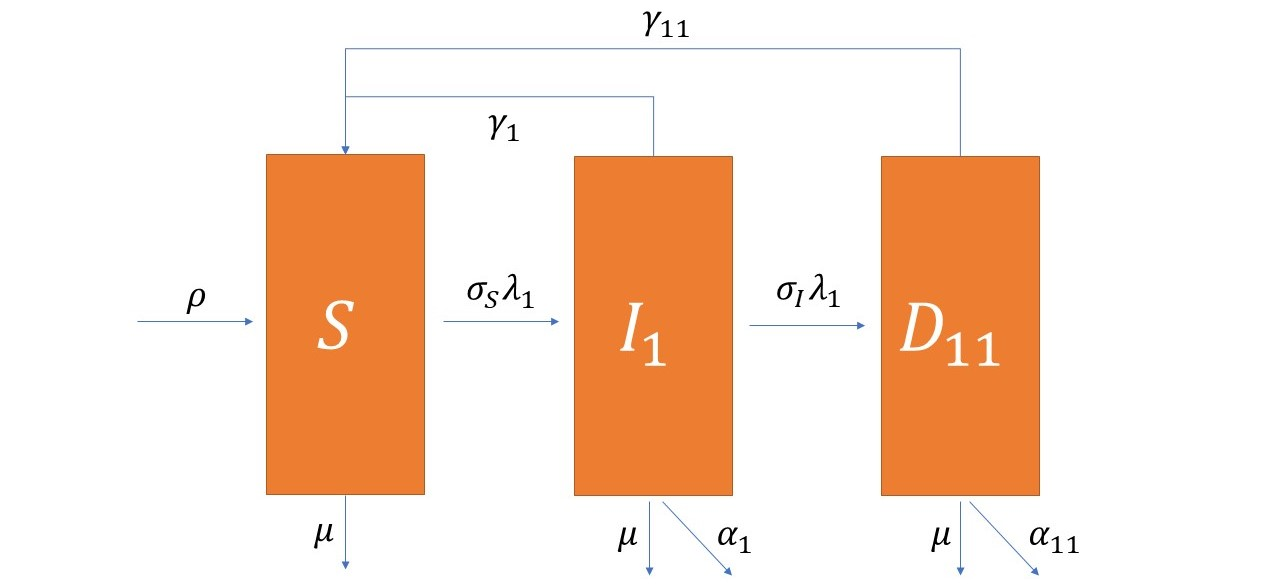
\includegraphics[width=230pt]{model_with_recovery.jpg}
			\end{center}
			\caption{Schematic diagram of the model with recovery.}
		\end{figure}
	\end{frame}

	\begin{frame}{Extension: Model with recovery}
		\begin{figure}[ht]
			\label{Figure 12}
			\begin{center}
				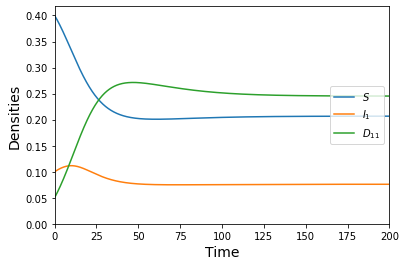
\includegraphics[width=240pt]{plot_dynamics_with_recovery.jpg}
			\end{center}
			\caption{Population dynamics in the model with recovery.}
		\end{figure}
		\begin{itemize}
			\item The scenarios in equilibrium are similar to the original model.
		\end{itemize}
	\end{frame}

	\begin{frame}
		\begin{figure}[htbp]
			\label{Figure 13}
			\centering
			\subfigure[]{
				\begin{minipage}{0.32\columnwidth}
					\centering
					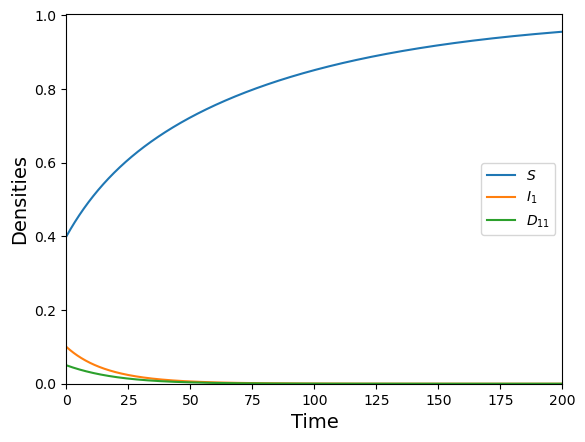
\includegraphics[width=111pt]{free_recovery_1.jpg}
				\end{minipage}
			}\subfigure[]{
				\begin{minipage}{0.32\columnwidth}
					\centering
					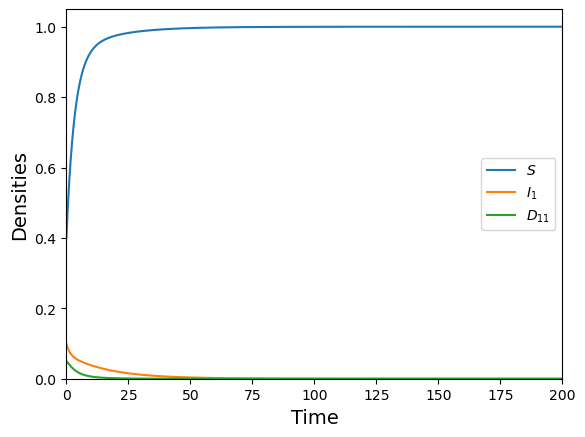
\includegraphics[width=111pt]{free_recovery_2.jpg}
				\end{minipage}
			}\subfigure[]{
				\begin{minipage}{0.32\columnwidth}
					\centering
					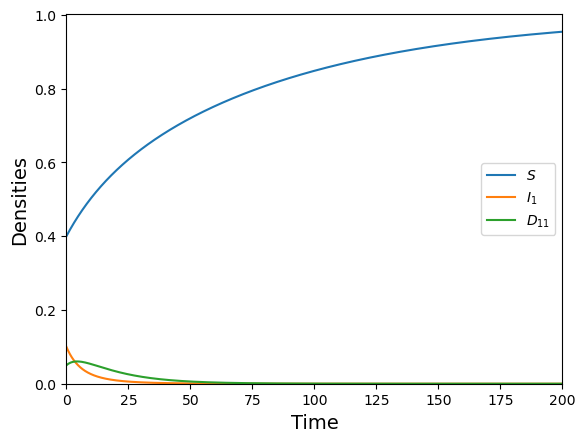
\includegraphics[width=111pt]{free_recovery_3.jpg}
				\end{minipage}
			}
			\qquad
			\subfigure[]{
				\begin{minipage}{0.32\columnwidth}
					\centering
					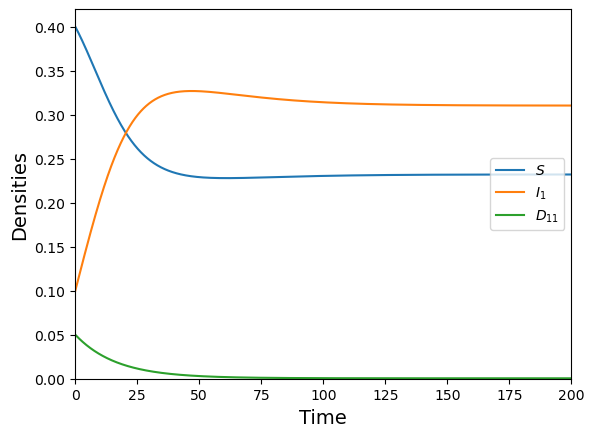
\includegraphics[width=111pt]{single_recovery.jpg}
				\end{minipage}
			}
			\caption{\tiny (a), (b), (c): disease-free case, with low transmission rate, high background mortality rate and low vulnerability of susceptible host, respectively; (d): Single-infection-only case with low vulnerability of infected hosts.}
		\end{figure}
	\end{frame}

	\section{References}
	\begin{frame}{References:}
		\scriptsize Alizon, S. (2013) ‘Co-infection and super-infection models in evolutionary epidemiology’, Interface focus, 3(6), pp. 20130031–20130031. doi:10.1098/rsfs.2013.0031.\\
		\vspace{1em}
		Boots, M. and Haraguchi, Y. (1999) ‘The Evolution of Costly Resistance in Host‐Parasite Systems’, The American naturalist, 153(4), pp. 359–370. doi:10.1086/303181.\\
		\vspace{1em}
		Cressler, C.E. et al. (2016) ‘The adaptive evolution of virulence: a review of theoretical predictions and empirical tests’, Parasitology, 143(7), pp. 915–930. doi:10.1017/S003118201500092X.\\
		\vspace{1em}
		De Roode, J.C. et al. (2005) ‘Dynamics of Multiple Infection and Within‐Host Competition in Genetically Diverse Malaria Infections’, The American naturalist, 166(5), pp. 531–542. doi:10.1086/491659.\\
		\vspace{1em}
		Francisco Jr, R. da S. et al. (2021) ‘Pervasive transmission of E484K and emergence of VUI-NP13L with evidence of SARS-CoV-2 co-infection events by two different lineages in Rio Grande do Sul, Brazil’, Virus research, 296, pp. 198345–198345. doi:10.1016/j.virusres.2021.198345.\\
		\vspace{1em}
		Van Baalen, M. and Sabelis, M.. (1995) ‘The Dynamics of Multiple Infection and the Evolution of Virulence’, The American naturalist, 146(6), pp. 881–910. doi:10.1086/285830.
	\end{frame}
\end{document}